\textbf{4-1} 长方形导体块如电图4-1-1所示。从 $t = 0$ 开始，外加与导体表面垂直的均匀电场 $\pmb{E}_0$，导体中开始有电流，导体两端的表面开始积累电荷。设 $\pmb{E}_0$ 并不太强，故导体中自由电子的数密度近似不变，从而导体的电导率 $\sigma$ 可视为常数。设电子运动到导体两端后就停留在表面上。导体的表面很大，边缘效应可以忽略。试求导体表面积累电荷的面密度 $\sigma_{\mathrm{e}}$ 及导体中电流密度 $j$ 随时间的变化。

本题为导体在外电场下达到静电平衡的过程提供了一种简化模型。
\begin{center}
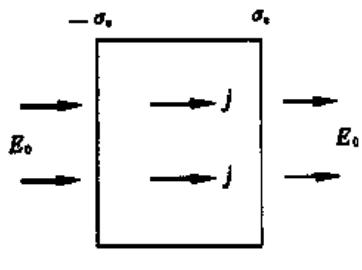
\includegraphics[width=0.2\textwidth]{figures/d7f80597ec698393942d6cf26dff9dc250dd24b7931ff95ba5265ebedb3043d4.jpg}
\end{center}
\vfill

\textbf{4-2} 如电图4-2-1所示，圆柱形电阻器的截面积为 $S$，长为 $2L$，电导率为
$$
\sigma = \begin{cases} \sigma_{0}\!\left(1 + \dfrac{x}{L}\right), & 0 < x < L \\[6pt] \sigma_{0}\!\left(1 + \dfrac{2x}{L}\right), & L < x < 2L \end{cases}
$$
在电阻器两端面之间加电压 $\Delta U$，电流恒定均匀地从一个端面流入，从另一端面流出。

试求：

1. 电阻器的电阻 $R$。

2. 电阻器中体电荷密度 $\rho_{e}$ 的分布（$x=L$ 处除外）。

3. 电阻器 $x = L$ 处的面电荷密度 $\sigma_{e}$。

\begin{center}
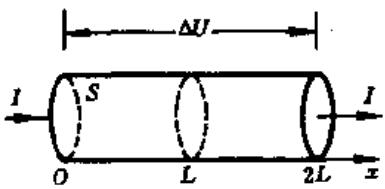
\includegraphics[width=0.25\textwidth]{figures/a075ff49a0e5756243a39b935177f3c480e5507177dc22bb24612fe7ef61f5a0.jpg}
\end{center}
\vfill

\newpage
\textbf{4-3} 天气晴朗时，地球大气中沿径向有正的体电荷密度 $\rho_{\mathrm{e}}(r)$ 分布，地球表面则有负的均匀面电荷密度 $\sigma_{e}$，这样，在大气中便有径向电场 $E(r)$，从而形成径向电流。已知大气的电导率分布为
$$
\sigma(r) = \sigma_{0} + a(r - R)^{2}
$$
式中 $\sigma_{0} = 3.0\times 10^{-14}\,\mathrm{1/(\Omega\cdot m)}$，$a = 0.5\times 10^{-20}\,\mathrm{1/(\Omega\cdot m^{3})}$，$R = 6\times 10^{6}\,\mathrm{m}$（地球半径）。$r$ 从地球中心算起，已知地球表面的电场强度为 $E(R) = -100\,\mathrm{V/m}$（负号表示电场强度指向地球中心）。设地球作为导体，其内部无电荷，并设大气中的体电荷密度 $\rho_{\mathrm{e}}(r)$ 及地球表面的电荷密度 $\sigma_{\mathrm{e}}$ 均不随时间变化（稳态近似），即大气中的径向电流是恒定的。

试求：1. 地球表面的总电流强度。

2. 地球表面的面电荷密度 $\sigma_{e}$。

3. 地球大气中体电荷密度的分布 $\rho_{\mathrm{e}}(r)$。4. 大气顶层与地球表面之间的电势差 $V$。
\vfill

\textbf{4-4} 如电图4-4-1所示，在 $0 \leqslant r < R_{1}$ 的球形区域内，充满了电容率为 $\varepsilon_{1}$、电导率为 $\sigma_{1}$ 的均匀介质。在 $R_{1} < r < R_{2}$ 的球壳状区域内，充满了电容率为 $\varepsilon_{2}$、电导率为 $\sigma_{2}$ 的另一种均匀介质。在 $R_{2}$ 之外为真空。设 $t = 0$ 时，自由电荷体密度的分布为
$$
\rho_{\mathrm{e}} = \begin{cases} \rho_{\mathrm{e0}}, & 0 \leqslant r < R_{1} \\ 0, & R_{1} < r < R_{2} \end{cases}
$$
且 $R_{1}$ 和 $R_{2}$ 两球面上自由电荷的面密度 $\sigma_{\mathrm{e}1}$ 和 $\sigma_{\mathrm{e}2}$ 均为零。试求 $\sigma_{\mathrm{e}1}$ 和 $\sigma_{\mathrm{e}2}$ 随时间 $t$ 变化的规律。
\begin{center}
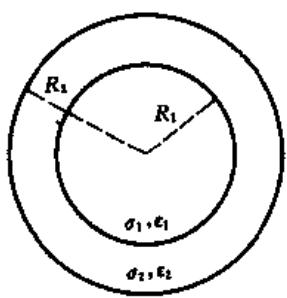
\includegraphics[width=0.2\textwidth]{figures/ce674ef7ec26fb78264954a709500272320b566ab7b95d8f92b7701aaf80c7df.jpg}
\end{center}
\vfill

\newpage
\textbf{4-5} 在电容率为 $\varepsilon$ 的某超导体内，正、负离子的质量分别为 $m_{+}$ 和 $m_{-}$，正、负离子的电量分别为 $q_{+}$ 和 $q_{-}$，平衡时正、负离子的电荷密度分别为 $\rho_0$ 和 $-\rho_0$。超导体是以 $x$ 轴为母线的柱体，且始终处于低温（接近 $T \approx 0\,\mathrm{K}$）之中。开始时超导体处于平衡状态，后来因为受到 $x$ 方向的扰动使离子有微小的运动。试证明，离子的这种小运动必定是简谐振动，并求出振动的圆频率。
\vfill

\textbf{4-6} $n$ 个电阻 $r$ 连成电阻为 $R$ 的系统，再将两个电阻 $r$ 与系统连接。试问连接后电阻值能否保持不变，即仍为 $R$。
\vfill

\newpage
\textbf{4-7} 将阻值分别为 $1\,\Omega, 2\,\Omega, 3\,\Omega, 4\,\Omega, 5\,\Omega, 6\,\Omega$ 的6个电阻连接成如电图4-7-1所示的电路。若已测得 $R_{XY} = 7\frac{3}{13}\,\Omega$，$R_{YZ} = 10\frac{1}{13}\,\Omega$，$R_{ZX} = 6\frac{9}{13}\,\Omega$。试求图中6个电阻 $a, b, c, d, e, f$ 各自的阻值。

\begin{center}
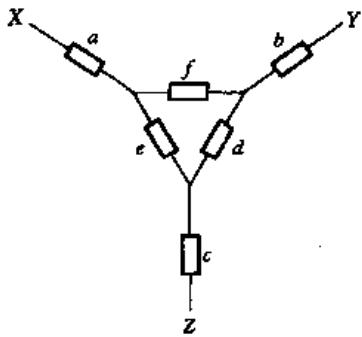
\includegraphics[width=0.25\textwidth]{figures/77abf5ee565396a1f413b0ef4fef9a6cab2927f7afb91fc9a5a4ae85784bda6f.jpg}
\end{center}
\vfill

\textbf{4-8} 有8个外观完全相同的电阻，其中7个阻值相同，另1个阻值与它们不同，称为"特殊的"电阻。试设计一种测量方案，要求只使用欧姆表三次，便可将该"特殊的"电阻检出。
\vfill

\newpage
\textbf{4-9} 正四面体框架形电阻网络如电图4-9-1所示，其中每一小段的电阻均为 $R$。试求：1. $A, B$ 两端点之间的等效电阻 $R_{AB}$。2. $C, D$ 两端点之间的等效电阻 $R_{CD}$。

\begin{center}
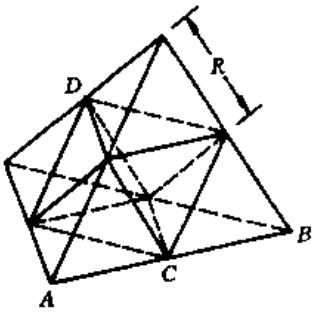
\includegraphics[width=0.2\textwidth]{figures/电图4-9-1.jpg}
\end{center}
\vfill

\textbf{4-10} 三个相同的均匀金属圆圈两两相交地连接成如电图4-10-1所示的网络，已知每一个金属圆圈的电阻都是 $R$。试求电图4-10-1中 $A, B$ 两点之间的等效电阻 $R_{AB}$。

\begin{center}
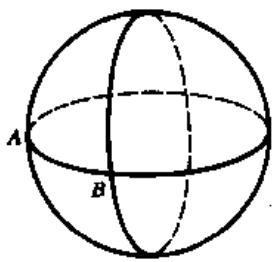
\includegraphics[width=0.2\textwidth]{figures/电图4-10-1.jpg}
\end{center}
\vfill

\newpage
\textbf{4-11} 二端无限梯形电阻网络如电图4-11-1所示，它由 $K \to \infty$ 个相同的网络元串接而成，每个网络元包含三个相同的电阻 $R$。通常采用极限法来计算 $A, B$ 两端点之间的等效电阻 $R_{AB}$。所谓极限法，就是先设 $K$ 个网络元组成二端网络，其等效电阻记为 $R_{K}$，再连接一个网络元，其等效电阻记为 $R_{K+1}$。设法找出 $R_{K+1}$ 与 $R_{K}$ 之间的递推关系，最后令 $K \to \infty$。

不难看出，上述做法是不够严谨的，因为只有证明数列 $R_{1}, R_{2}, \cdots, R_{K}, \cdots$ 存在极限 $R_{\infty}$ 之后，才有 $K \to \infty$ 时，$R_{K+1} = R_{K} = R_{\infty} = R_{AB}$ 的结果。换言之，不能"想当然"地认为，$K \to \infty$ 时，一定有 $R_{K+1} = R_{K} = R_{\infty}$ 的结果。

为了在严格的意义上讨论 $A, B$ 之间的等效电阻 $R_{AB}$，特编制以下各题，试逐一予以解答。

1. 在找出数列 $R_{K}$ 的数学表达式之前, 试定性证明 $\{R_{K}\}$ 是一个单调递减的有界数列, 因此存在极限.

2.(a)试导出 $R_{K - 1}(R_K)$ 递推关系式.

(b)试由上述递推关系式,解出 $R_{K}(R)$ 表达式.

(c)试由 $R_{K}(R)$ 表达式定量证明 $\{R_K\}$ 是一个单调递减的有界数列，因此存在极限.

(d)试求出 $R_{K}$ 的极限，即 $R_{AB}$ 值.

最后,需要指出,在求解二端无限网络的等效电阻问题时,一般说来,若题文中无特殊要求,即意味着该题存在极限,解题者可在此基础上求解,不必作如本题的严格论证.

\begin{center}
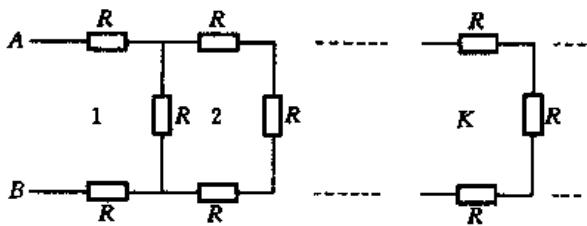
\includegraphics[width=0.3\textwidth]{figures/电图4-11-1.jpg}
\end{center}
\vfill
\newpage

\textbf{4-12} 如电图4-12-1所示是由电阻丝连接成的无限电阻网络，已知每一段电阻丝的电阻均为 $r$。试求 $A, B$ 两点之间的等效电阻 $R_{AB}$。

\begin{center}
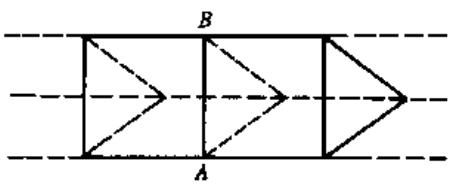
\includegraphics[width=0.3\textwidth]{figures/电图4-12-1.jpg}
\end{center}
\vfill

\textbf{4-13} 由7个阻值均为 $r$ 的电阻组成的网络元如电图4-13-1所示。由这种网络元彼此连接构成的二端无限网络，试求两端之间的等效电阻。

\begin{center}
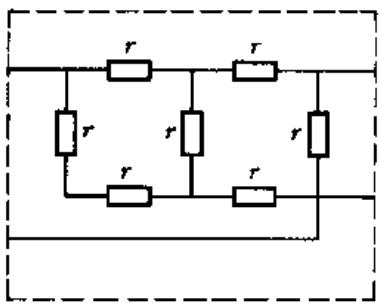
\includegraphics[width=0.3\textwidth]{figures/电图4-13-1.jpg}
\end{center}
\vfill
\newpage


\textbf{4-14} 用同种均匀金属丝连接成的无限内接等边三角形电阻网络如电图4-14-1所示，每个外三角形的三边中点为内接三角形的三个顶点。设最外面的等边三角形的边长为 $a$，金属丝单位长度的电阻为 $r$，试求 $A,B$ 之间的等效电阻 $R_{AB}$。

\begin{center}
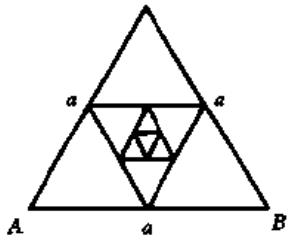
\includegraphics[width=0.2\textwidth]{figures/电图4-14-1.jpg}
\end{center}
\vfill


\textbf{4-15} 10根电阻均为 $R$ 的电阻丝连接成如电图4-15-1所示的电阻网络，试求 $A, B$ 两点之间的等效电阻 $R_{AB}$。

\begin{center}
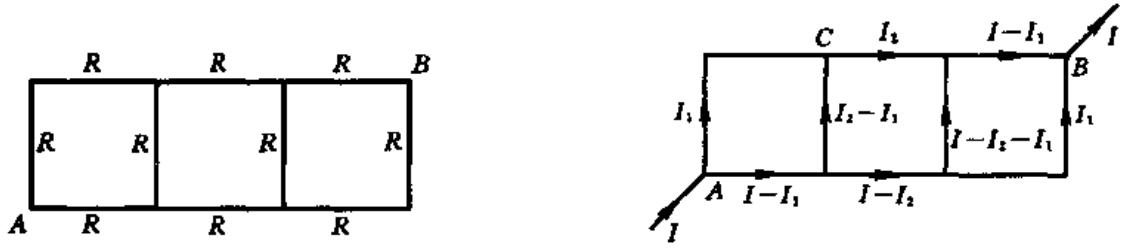
\includegraphics[width=0.6\textwidth]{figures/电图4-15-1.jpg}
\end{center}
\vfill
\newpage

\textbf{4-16} 如电图4-16-1所示的电阻丝网络包含 $N \geqslant 3$ 个正方形，网络中每一小段的电阻均为 $R$。试求 $A, B$ 之间的等效电阻 $R_{AB}$。

\begin{center}
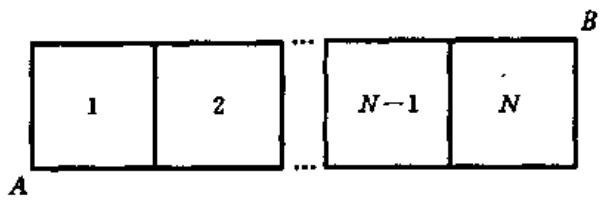
\includegraphics[width=0.3\textwidth]{figures/电图4-16-1.jpg}
\end{center}
\vfill


\textbf{4-17} 电阻丝网络如电图4-17-1所示，每一小段的电阻均为 $R$。试求 $A, B$ 之间的等效电阻 $R_{AB}$。

\begin{center}
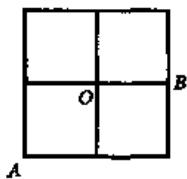
\includegraphics[width=0.2\textwidth]{figures/电图4-17-1.jpg}
\end{center}
\vfill
\newpage

\textbf{4-18} 电阻丝构成的圆环分格（格数 $n \geqslant 2$）网络如电图4-18-1所示，其中每段电阻丝的电阻均为 $R$。试求 $A, B$ 两节点之间的等效电阻 $R_{AB}$。

\begin{center}
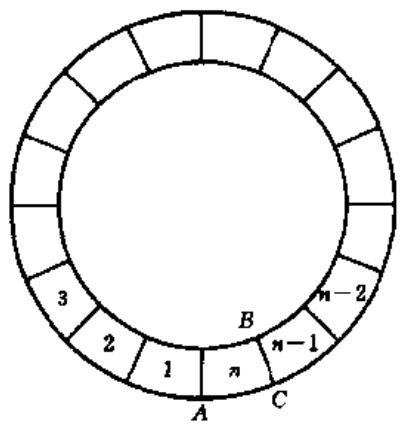
\includegraphics[width=0.2\textwidth]{figures/电图4-18-1.jpg}
\end{center}
\vfill


\textbf{4-19} 试求平面正方形无穷电阻网络任意两节点之间的等效电阻。已知网络中各小段电阻均为 $r$。并推广到其他类型的无穷电阻网络，如平面矩形网络，平面正三角形网络，平面正六角形网络，三维立方体网络等，试求这些无穷电阻网络任意两节点之间的等效电阻。
\vfill
\newpage

\textbf{4-20} 如果电图4-20-1中两个电路之间具有这样的对应关系：当电路(ii)中 $a, b, c$ 端的电势分别与电路(i)中 $A, B, C$ 端的电势相同时，从 $a, b, c$ 端流入的电流便分别与从 $A, B, C$ 端流入的电流相同。若电路(i)中的三个电阻 $R_{AB}, R_{BC}, R_{CA}$ 为已知，试求电路(ii)中的 $R_a, R_b, R_c$。

\begin{center}
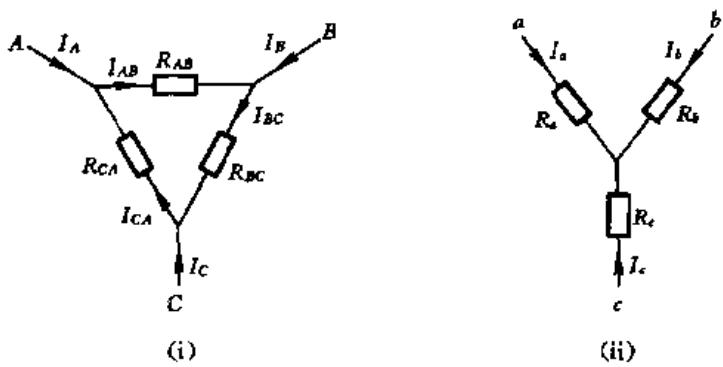
\includegraphics[width=0.4\textwidth]{figures/电图4-20-1.jpg}
\end{center}
\vfill


\textbf{4-21} 某含源二端网络，其输出的伏安特性曲线具有负斜率。试分析此二端网络的内阻特点。
\vfill
\newpage

\textbf{4-22} 如电图4-22-1所示的立方体网络中，每一小段直线的电阻均为 $R$，试求 $R_{PQ}$。

\begin{center}
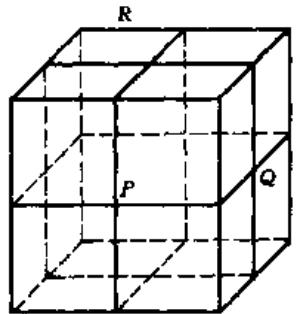
\includegraphics[width=0.2\textwidth]{figures/电图4-22-1.jpg}
\end{center}
\vfill


\textbf{4-23} 电灯泡的电阻为 $R_0 = 2\,\Omega$，正常工作电压为 $U_{0} = 4.5\,\mathrm{V}$，用电动势 $U = 6\,\mathrm{V}$ 且内阻可以忽略的电池供电，并利用一滑线电阻器将灯泡与电池相联。试求效率为最大的条件及最大效率值。又为使系统的效率不低于 $\eta = 0.6$，试计算电阻器的阻值及其承受的最大电流。
\vfill
\newpage

\textbf{4-24} 1. 在如电图4-24-1所示的电路中，各个电阻的阻值都是 $1\,\Omega$，安培计与电源的内阻均可忽略不计，电源的电动势 $\varepsilon = 10\,\mathrm{V}$。试求通过安培计的电流强度。

\begin{center}
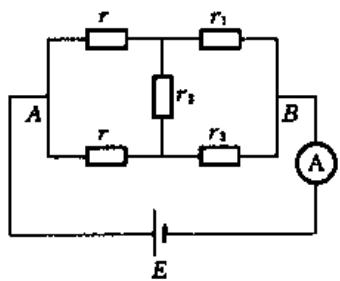
\includegraphics[width=0.2\textwidth]{figures/bb27fccee51963a9e3feaa4f4d44e130952672bd63cf5577658d69c00c16665b.jpg}
\end{center}

2. 若图中的两个 $r$ 是好电阻，而 $r_1, r_2, r_3$ 是三个坏电阻，它们互不相关地时通、时断，已知 $r_1, r_2, r_3$ 各自通电的概率都是 $\frac{1}{2}$。试求电源的平均输出功率。
\vfill


\textbf{4-25} 为使如电图4-25-1和电图4-25-2所示的两个电路中，流过任意具有相同阻值的外电阻 $R$ 的电流 $I$ 相同。试求电源 $(\mathcal{E}, r)$ 与电源组 $(\mathcal{E}_1, r_1), (\mathcal{E}_2, r_2)$ 之间的定量关系，其中符号 $\mathcal{E}$ 和 $r$ 分别表示电源的电动势和电阻。

\begin{center}
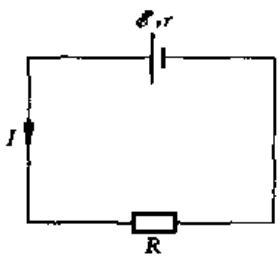
\includegraphics[width=0.25\textwidth]{figures/电图4-25-1.jpg}
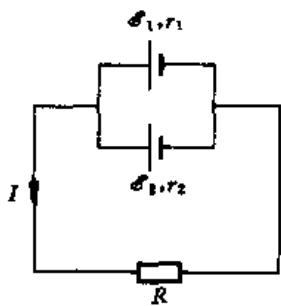
\includegraphics[width=0.25\textwidth]{figures/电图4-25-2.jpg}
\end{center}

\vfill
\newpage

\textbf{4-26} 如电图4-26-1所示为一惠斯通电桥，电路参量为 $R_{1} = R_{2} = R_{3} = R_{4} = 10.000\,\Omega$，电流计G的内阻为 $R_{g}$，电池内阻可略，电动势为 $\varepsilon = 2.000\,\mathrm{V}$。

1. 在 $R_{g} = 0$ 和 $R_{g} = \infty$ 两种情况下，试计算线路中 $A$ 和 $B$ 两点之间的等效电阻。

2. 设电桥四臂电阻参量确如上述，试证明合上电键 K 后，无论 $R_{g}$ 取何值，均无电流流过电流计 G。

\begin{center}
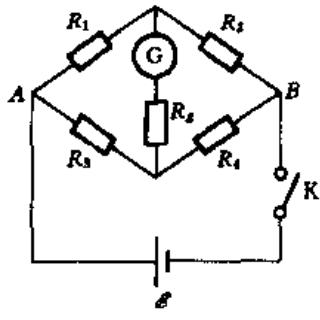
\includegraphics[width=0.2\textwidth]{figures/电图4-26-1.jpg}
\end{center}
\vfill


\textbf{4-27} 在如电图4-27-1所示的电路中，$R_{1}, R_{2}, \cdots, R_{g}$ 均为阻值有限的电阻，电流计G连同其串联电阻 $R_{g}$ 接在B和F之间。若定义 $\alpha$ 和 $\beta$ 为
$$
\alpha = \frac{R_{1}}{R_{6}}, \quad \beta = \frac{R_{2} + R_{3}}{R_{4} + R_{5}}
$$
试证明，当 $R_{5}=0$ 时，无电流流过电流计的必要条件是 $\alpha=\beta$。

\begin{center}
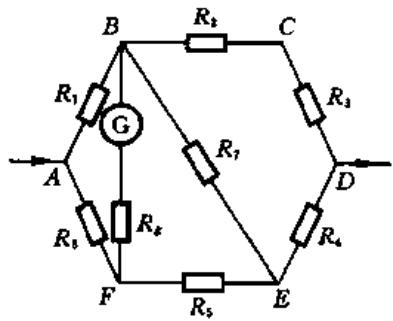
\includegraphics[width=0.25\textwidth]{figures/电图4-27-1.jpg}
\end{center}
\vfill
\newpage

\textbf{4-28} 试证明在平衡电桥中，电桥臂上的微小电阻变化所引起的检流计读数的微小偏转是线性的。即试证明检流计偏转角与臂电阻微小变化量成正比。
\vfill


\textbf{4-29} 有若干个电阻构成如电图4-29-1所示的电路,其中 A 和 B 两点的接地电阻是固定不动的.输入电压 $V_{1}, V_{2}, \cdots, V_{n}$ 仅取 $1 V$ 或 $0 V$ 两个值,$0 V$ 表示接地.试问 B 点的最大输出电压是多少?
\begin{center}
    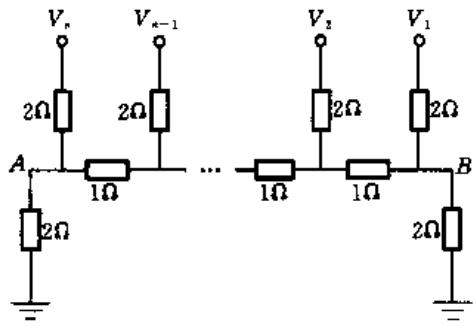
\includegraphics[width=0.25\textwidth]{figures/电图4-29-1.jpg}
    \qquad
    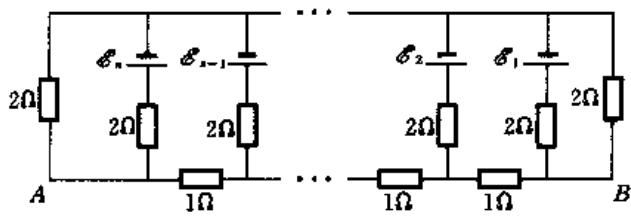
\includegraphics[width=0.25\textwidth]{figures/电图4-29-2.jpg}
\end{center}

\vfill
\newpage

\textbf{4-30} 在如电图4-30-1所示的电容网络中，已知 $C_1 = C_2 = C_3 = C_9 = 1\,\mu\mathrm{F}$，$C_4 = C_5 = C_6 = C_7 = 2\,\mu\mathrm{F}$，$C_8 = C_{10} = 3\,\mu\mathrm{F}$。试求 $A, B$ 两点之间的等效电容 $C_{AB}$。

\begin{center}
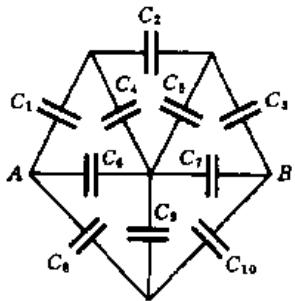
\includegraphics[width=0.2\textwidth]{figures/电图4-30-1.jpg}
\end{center}
\vfill


\textbf{4-31} 如电图4-31-1所示，左边的三端电容网络为 $\triangle$ 型网络元，右边的三端电容网络为 $Y$ 型网络元，试导出其间的等效变换公式。

然后，利用上述等效变换，试计算电图4-31-2所示电容网络中A和B两点之间的等效电容 $C_{AB}$。电图4-31-2网络中各电容已用数字标明，单位均为 $\mu\mathrm{F}$。

\begin{center}
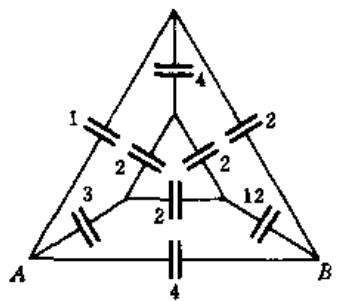
\includegraphics[width=0.2\textwidth]{figures/电图4-31-2.jpg}
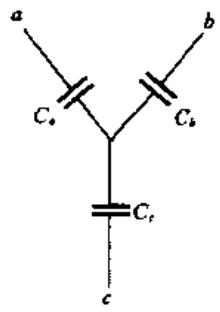
\includegraphics[width=0.15\textwidth]{figures/电图4-31-1.jpg}
\end{center}
\vfill
\newpage

\textbf{4-32} 用由 $N$ 个相同的电池串联而成的电池组对一电容器充电。第一种充电方式是将此电容器与一电阻串联后，接在 $N$ 个串联电池的两端。第二种充电方式是将此电容器与同一电阻串联后，先用一个电池充电，接着改用两个串联电池继续充电，再改用三个串联电池继续充电，$\cdots$，最后用 $N$ 个串联电池为其充电（即逐个添加电池，不断继续充电，直至 $N$ 个串联电池为其充电结束）。试问这两种充电方式的电能损耗是否相同？若不相同，哪种充电方式损耗的电能较多？
\vfill


\textbf{4-33} 在如电图4-33-1所示的由电容和直流电源构成的网络中，$C_1 = 4C_0, C_2 = 2C_0, C_3 = C_0$，电源电动势为 $\mathcal{E}$，电源内阻可忽略不计。先断开 $\mathbf{k}_4$，接通 $\mathbf{k}_1, \mathbf{k}_2, \mathbf{k}_3$，为三个电容器充电。尔后断开 $\mathbf{k}_1, \mathbf{k}_2, \mathbf{k}_3$，接通 $\mathbf{k}_4$，使电容器放电。

试求放电过程中流过某一特定电容器的总电量。

\begin{center}
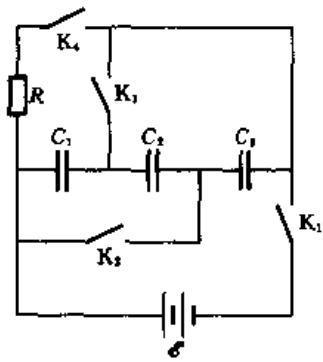
\includegraphics[width=0.2\textwidth]{figures/电图4-33-1.jpg}
\end{center}
\vfill
\newpage

\textbf{4-34} 由 $n$ 个网络元组成的电容网络如电图4-34-1所示，每一个网络元由三个电容器连接而成，其中上、下两个电容器的电容均为 $3C$，右侧电容器的电容均为 $2C$。电图4-34-1中的 $a$ 和 $b$ 点是网络的输入端，$a'$ 和 $b'$ 点是网络的输出端，在 $a$ 和 $b$ 之间有恒定的输入电压 $U$，在 $a'$ 和 $b'$ 之间连接一个电容为 $C$ 的电容器。

1. 试求从第 $k(k<n)$ 个网络元的输入端算起，后面所有电容器贮存的总电能。

2. 先将第1个网络元的输出端与其右侧的网络断开，再除去电源，并把它的输入端 $a$ 和 $b$ 连接起来。试求这时构成第1个网络元的三个电容器中贮存的总电能。

\begin{center}
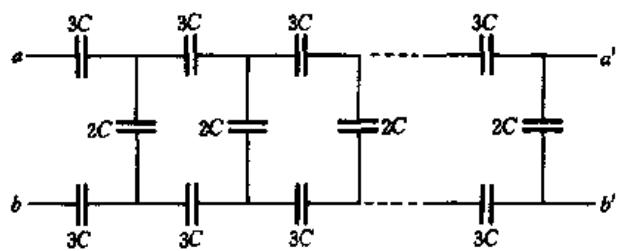
\includegraphics[width=0.3\textwidth]{figures/电图4-34-1.jpg}
\end{center}
\vfill

\textbf{4-35} 如电图4-35-1所示，12根电阻均为 $R$ 的电阻丝连接成正六面体（立方体）。在两根电阻丝中连有电动势分别为 $\mathcal{E}_1$ 和 $\mathcal{E}_2$ 的电源，另5根电阻丝中连有5个相同的电容器 $C$。设电源正、负极之间的距离均可忽略，内阻亦可略，且 $\mathcal{E}_1 = 2I_0R, \mathcal{E}_2 = I_0R$。试求：1. AB中的电流 $I_{AB}$。2. $A^{\prime}B^{\prime}$ 中电容器极板上的电量 $Q_{A'B'}$。

\begin{center}
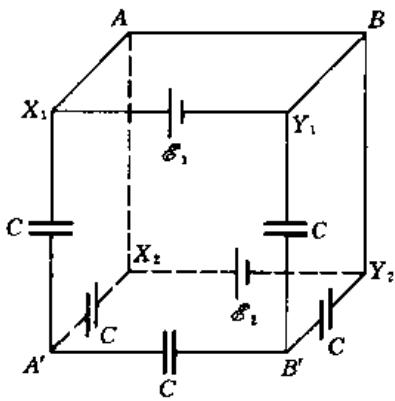
\includegraphics[width=0.2\textwidth]{figures/电图4-35-1.jpg}
\end{center}
\vfill

